\chapter*{Annexe 1
\\RESTful Web Services}
\addcontentsline{toc}{chapter}{Annexe 1}
\makeatletter
\renewcommand{\thesection}{\@arabic\c@section}
\makeatother
\renewcommand\thefigure{\thesection.\arabic{figure}}    
\setcounter{figure}{0}

\renewcommand\thetable{\thesection.\arabic{table}}    
\setcounter{table}{0}
%recommencer la numérotation des section à "1"
\setcounter{section}{0}

\qquad Representational State Transfer ou communément REST est une architecture d'application basée sur le standard HTTP. REST utilise les opérations natives de HTTP : POST, GET, PUT, DELETE pour le mapping sur les quatre fonctions fondamentales d'une base de données qui sont Create, Read, Delete, et Update. Ces services peuvent ensuite être consommés par des clients authentifiés \cite{7}.\\

Les services Web REST sont utilisés pour développer des applications orientées ressources dans lesquelles chaque composant est une ressource accessible en utilisant les méthodes standards du HTTP. Les applications qui respectent les architectures orientées ressources sont appelées RESTful.

\section{Caractéristiques}

\begin{itemize}
	\item Sans état : le serveur ignore l'état des clients entre les requêtes
	\item Cacheable : les candidats doivent être capables de garder en mémoires des informations.
	\item Orienté clients serveur : le client et le serveur sont les entités communiquent dans une architecture REST. Le client requière une ressource et le serveur la lui fournira, s'il est authentifié.
	\item Réalisé en couche : le pattern MVC doit être respecté.
	\item Les ressources sont accessibles à travers les méthodes du HTTP (POST, GET, PUT, DELETE)\\
\end{itemize}

La communication entre le serveur et les clients peut se faire sous plusieurs formats : JASON, XML, CSV... Le présent projet utilise le format JSON pour la communication client-serveur.

\section{Méthodes du HTTP}

\begin{itemize}
	\item GET Accès en lecture seule à la ressource,
	\item PUT Création d’une nouvelle ressource,
	\item DELETE Suppression d’une ressource,
	\item POST Création d’une nouvelle ressource ou mise à jour d’une ressource existante
\end{itemize}

\begin{table}[!h]
	\caption{Exemple d’une API REST}
	\begin{tabular}{|L{3cm}|L{3cm}|L{4cm}|L{3cm}|}
		\hline
		Méthode HTTP & Route & Description & Type de l'opération\\
		\hline
		\hline
		GET & /Utilisateur/one & Obtenir un Utilisateur & lecture seule\\
		\hline
		GET & /Utilisateur/all & Obtenir tous les Utilisateurs & lecture seule\\
		\hline
		POST & /Utilisateur/add & Ajouter un Utilisateur & écriture seule\\
		\hline
		PUT & /Utilisateur/update & Mettre à jour un Utilisateur & écriture seule\\
		\hline
		DELETE & /Utilisateur/delete & Supprimer un Utilisateur & écriture\\
		\hline  
	\end{tabular}
	
\end{table}

\pagebreak

\section{Format de données}

Les différentes parties de notre application communiquent en utilisant le format de représentation de données JSON (JavaScript Object Notation – Notation Objet issue de JavaScript) qui est un format léger d'échange de données. Il est facile à lire ou à écrire pour des humains. 

JSON possède deux structures de données :
\begin{itemize}
	\item Objet : collection de pairs nom/valeur
	\item Liste : liste de valeurs ordonnés
\end{itemize}

la figure \ref{figB1} représente les deux structures de données JSON.\\

\begin{figure}[!h]
	\begin{center}
		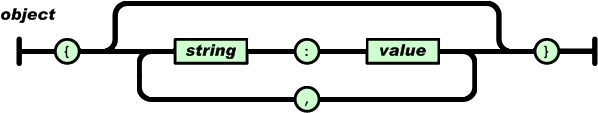
\includegraphics[width=14.7cm]{figures/object.png}
		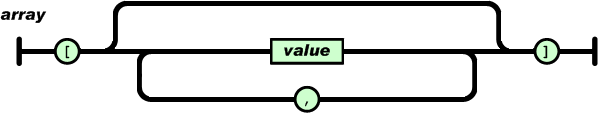
\includegraphics[width=14.7cm]{figures/array.png}
	\end{center}
\caption{Structures de données JSON}
%\source{Présentation de JSON\cite{bib12}}
\label{figB1}
\end{figure}
\newpage
\subsection{Exemple}
\textbf{paramètre de la requête d'un level :}

\begin{figure}[!h]
	\begin{center}
		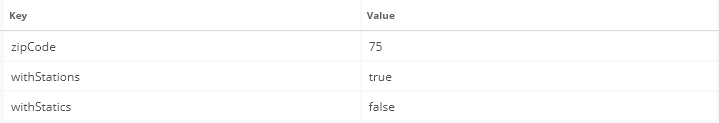
\includegraphics[width=14cm]{figures/param.png}
	\end{center}
	\caption{Paramètres d'une requête}
	\label{figB2}
\end{figure}

\textbf{Réponse du serveur :}

\begin{figure}[!h]
	\begin{center}
		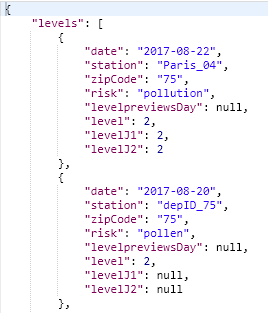
\includegraphics[width=6cm]{figures/reponse.png}
	\end{center}
	\caption{Réponse du serveur}
	\label{figB3}
\end{figure}

 